Turning to the profile of each cluster identified by the \dlearnerabbr{} model, Figure~\ref{fig:baseline-heatmap} shows the proportion of \diis{} in each identified cluster, and Figure~\ref{fig:baseline-heatrev} shows the proportion of sentences clustered together. In other words, Figure~\ref{fig:baseline-heatmap} shows whether each cluster mostly consists of one clause type, and Figure~\ref{fig:baseline-heatrev} shows whether each clause type is put in one cluster.  



\begin{figure}[H]
    \centering
    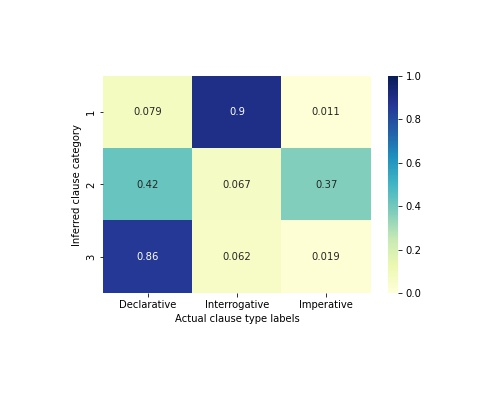
\includegraphics[width=0.7\textwidth]{figures/baseline-heatmap.jpg}
    \caption{The proportion of \diis{} in each of the three clusters identified by the \dlearnerabbr{} model}
    \label{fig:baseline-heatmap}
\end{figure}


\begin{figure}[H]
    \centering
    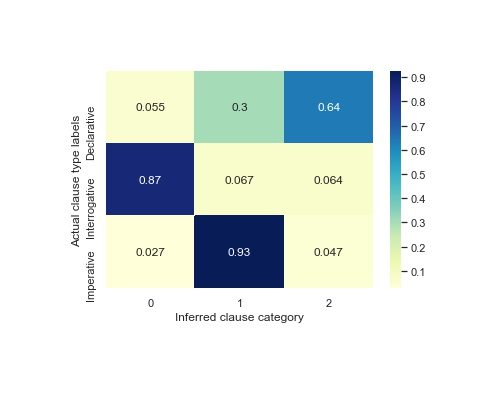
\includegraphics[width=0.7\textwidth]{figures/baseline-heatrev.jpg}
    \caption{The proportion of actual \diis{} clustered in one category}
    \label{fig:baseline-heatrev}
\end{figure}


Overall, Figure~\ref{fig:baseline-heatmap} shows that the \dlearnerabbr{} model identifies an interrogative cluster and a declarative cluster. Cluster~$0$ mostly contains interrogative clauses, as 90\% of sentences in this cluster are interrogative; Cluster~$2$ is mostly declarative, and 86\% of the data in this cluster are declaratives. Cluster~$1$ is split between declaratives and imperatives. Figure~\ref{fig:baseline-heatrev} shows that 87\% of interrogatives and 93\% of imperatives are clustered together in Cluster~$0$ and $1$ respectively. While most of declaratives are classified in Cluster~$2$, a proportion is classified in Cluster~$1$.

These results seem to suggest that the \dlearnerabbr{} found two out of three clause types, but how do these clause types look like? Did the model find the right morpho-syntactic properties to associate with each clause type? Figure~\ref{fig:baseline-syncluster} plots the morpho-syntactic profile of each cluster identified by the \dlearnerabbr{}. Darker colors represent sentences with the morpho-syntactic property, and lighter colors represent sentences without the property. 

\begin{figure}[H]
    \centering
    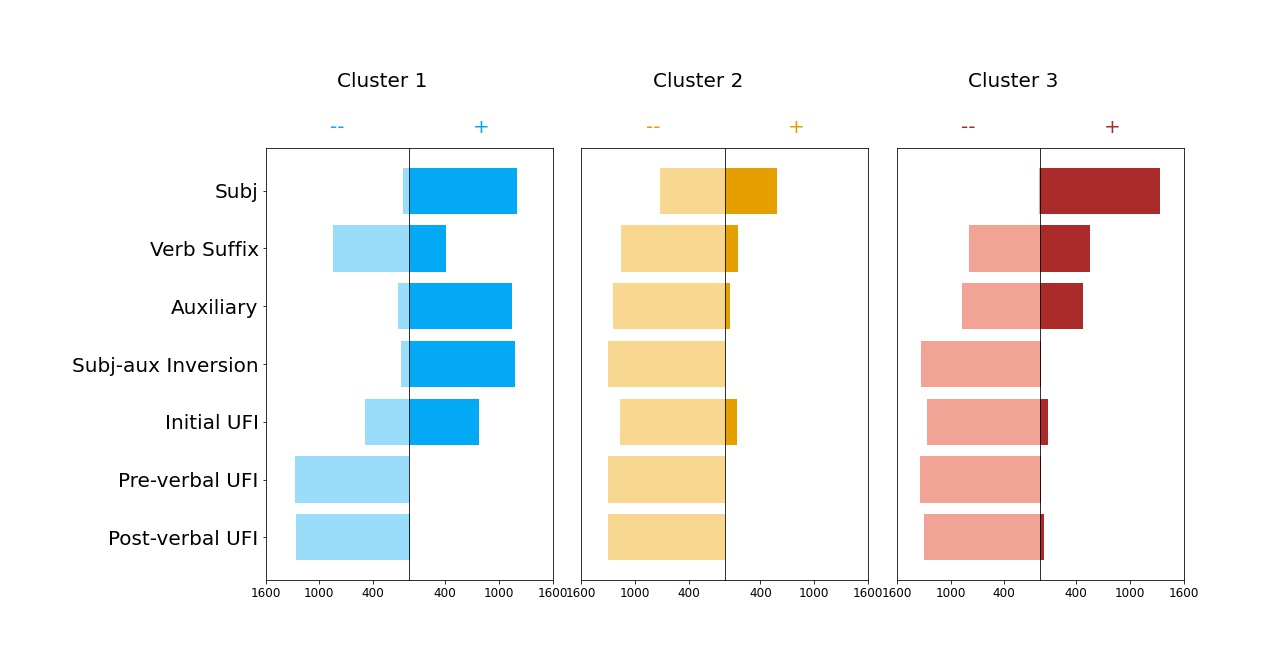
\includegraphics[width=1\textwidth]{figures/baseline-syncluster.jpg}
    \caption{The number of sentences with/without certain formal features in each cluster (Cluster 0 $\sim$ Interrogatives, Cluster 1 $\sim$ Imperatives, Cluster 2 $\sim$ Declaratives), darker colors represent the number of sentences with the feature. UFI stands for Unknown Functional Item (e.g. \twh{}), see Table~\ref{tab:eng-cl:formal-schema} for details.}
    \label{fig:baseline-syncluster}
\end{figure}

We can see that Cluster~$0$, which is 90\% interrogative clauses, is associated with [+int] morpho-syntactic properties such as subject-auxiliary inversion and sentence-initial unknown functional item (e.g. \twh{}). 

The other two clusters are not as ideal. Cluster~$1$ consists of a mix of imperative sentences and simple declarative sentences. While it appears that the cluster mostly consists of sentences with bare verb stem, which is characteristic for imperatives in English, but a quick look at the sentences show that it also includes declaratives with these properties as well:

\bex{engcl:baseline:cluster1-dec}
\ex I love school. \hfill Mother of Lily, Session 010423
\eex

The sentence is clustered together with imperatives like \tit{Take the bottle!} by the model. Ambiguous sentences like \ref{engcl:baseline:cluster1-amb} are also put in this cluster:
\bex{engcl:baseline:cluster1-amb}
Wanna read your little Tigger book? \hfill Mother of Violet, Session 010407
\eex

Moreover, compare to the distribution of morpho-syntactic features of imperatives in English in Figure~\ref{fig:real-syncluster}, this cluster seems to have more sentences with subjects. It seems that instead of finding a cluster for imperatives and declaratives, the model finds a cluster of bare verb sentences that allows pro-drop, and a cluster of sentences that do not allow pro-drop. 

\begin{comment}
A multinomial logistic regression model was performed to further probe into the morpho-syntactic profile of each cluster, with the three
clusters as dependent variable (with Cluster~$2$ as the default), and the set of morpho-syntactic properties as independent variable. The results are shown in Table~\ref{tab:baseline-synstats} (details of the regression model, coefficients, and $p$-values are reported in Appendix~\ref{appx:engcl}).


\begin{table}[H]
\begin{center}
\begin{tabular}{c|p{10cm}}
\hline
Clusters (default Cluster~$2$) & Morpho-syntactic cues\\
\hline \hline
Cluster~$0$ & +auxiliary, +subject-auxiliary inversion, +sentence-initial UFI\\
\hline
Cluster~$1$  & $-$subject, $-$verb suffix\\
\hline \hline
\end{tabular}
\end{center}
\label{tab:baseline-synstats}
\end{table}%

The table shows that while 
\end{comment}

Overall, the \dlearnerabbr{} model fails to identify the clause type clustering in English, and fails to identify the characteristic morpho-syntactic properties for these clause types. 

